\section{Receiver Architecture}

\begin{figure}[h]
   \centering
    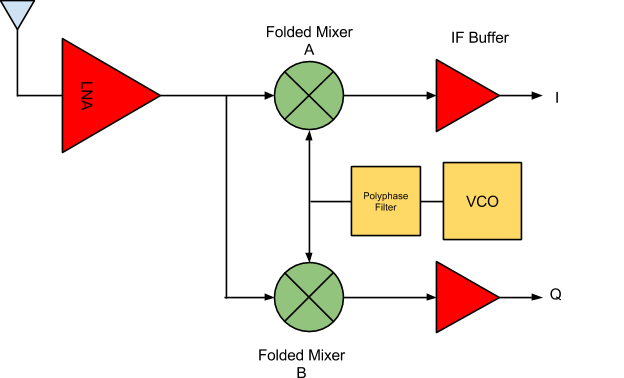
\includegraphics[width=0.55\textwidth]{figures/receiver}
    \caption{
        Block diagram of our low-IF receiver architecture. Folder mixers A and B are meant to implement quadrature downconversion. Due to time constraints, only the LNA, mixer A, and the VCO were fully implemented and integrated.
    }
    \label{fig:receiver}
\end{figure}

We considered several different architectures so as to make an informed decision as to what would be the best choice for the receiver. Our final choice was the low-IF architecture, but we will include what demotivated us towards selecting the other available ones. Primarily, we referred to Razavi~\cite{Razavi} when studying each architecture choice.


\subsection{Receiver Tradeoffs}
\subsubsection{Direct Conversion}
We have a channel bandwidth of 300 kHz in the 402-405 MHz core band and 100 kHz in the 401-402 MHz, 405-406 MHz sidebands. This channel bandwidth being downconverted directly would expose it to damaging flicker noise since CMOS technology is the primary circuit component in the LNA, filter, et cetera. Additionally, there are DC offset	 and local oscillator leakage problems that will contribute further to signal degradations.

\subsubsection{Super Regenerative}
Super regenerative receiver architectures have very good gains for the frequency range MedRadio operates at but requires a low number of interferers from neighboring bands and channels. The positive feedback architecture can serve to amplify noise to an unstable degree. As such, it suffers from poor selectivity, sensitivity (can be from 5-20 dB lower than heterodyne architectures), data rates, and has limited demodulation capability. 

\subsubsection{Dual-IF} 
Dual down conversion allows for both good channel selection and image rejection. However, multiple mixers increase the complexity of the circuit layout and requires additional band select, image reject, and channel selection components along the chain. This makes it difficult to manage reasonable linearity with good noise, power dissipation, and gain. So this won’t work for our application either. Also,  we want to avoid as many mixing spurs as possible and multiple image problems.

\subsubsection{Zero-Second IF}
This fixes the secondary image problem from Dual-IF but doesn’t fix the other issues. Additionally, it operates in the baseband -- where the flicker noise is the highest! This is unfeasible for us.

\subsection{Target Architecture: Low-IF}
Low-IF is an optimal choice for this type of application. The spectrum can be downconverted to a point where the Q factor is much lower and circuits can be designed using lower, optimal values. Downconverting the signal to a low frequency that isn't inside of the baseband (as in zero-IF) can help to avoid degradation from flicker noise of the MOSFETs.  Additionally, there is better frequency isolation in this architecture because the IF frequency can be selected such that the difference between the local oscillator (LO) frequency and the RF frequency is quite small. 

The downsides to this selection is that there are tradeoffs betwen image rejection and channel selection. High-IF implementations causes substantial image rejection since the image would be far outside of the bandwidth of the image-reject filter. However, this allows for close-by interferers to be allowed in with the spectrum of interest. Similarly, low-IF implementations cause substantial channel rejection by narrowly selecting the spectrum but allowing in images that are nearby to be downconverted to the same point. This issue, however,  can be fixed by implementing quadrature downconversion after the mixer.